\section{Introduction}
When a financial decision system trades, its actions can change the prices on which later decisions depend. Endogenous distribution shift denotes this feedback: the data-generating environment changes partly because of the system's own behavior. The statistical problem is therefore broader than predicting an outcome in a fixed historical dataset. One must distinguish a response observed under the historical environment from a response to an environment changed by the policy being evaluated.

This distinction is particularly important when expanding a deployed system into a population of hypothetical models. Perturbing an existing decision can support a sensitivity experiment. It cannot establish how a different language model would respond without original inputs, reproducible inference, and a validated response mapping. Likewise, agreement on a financial label is neither an accuracy measure nor a direct measure of systemic risk.

We study the gap between these evidence levels. Our contribution consists of an operational audit of \systemname{}, a common-input analysis of four exported model labels, and a reproducible single-asset simulation with paired participation and shock contrasts. The simulation is an explicitly chosen mechanism, not a calibrated replica of a real exchange. Its scientific result is conditional: participation can change both baseline drawdown and shock sensitivity, and the direction depends on the assumed response profile. A profile combining stronger selection and drawdown aversion does not yield a universal resilience benefit.

The study has three questions. What can the available operational records reconstruct? How different are the exported directional responses on a common panel? Within a specified price-feedback mechanism, how does changing allocated adaptive capital alter drawdown with and without an external shock? These questions are answered separately so that data provenance limitations do not become hidden assumptions in the simulation.

\section{Related work and scope}
Performative prediction formalizes how deployment can change the distribution on which a predictor is evaluated \citep{perdomo2020performative}. We use this motivation without claiming a new equilibrium theorem or empirical identification of performative stability. Our measured contrasts concern a finite simulation horizon and a chosen mechanism.

ABIDES provides an exchange-oriented discrete-event environment with explicit messages and configurable latencies \citep{byrd2019abides}. The present simulator is deliberately smaller: a single asset trades against an external dealer through aggregate price impact. Its transparent accounting enables controlled sensitivity analysis, but it does not reproduce matching-engine microstructure. These environments address different levels of fidelity.

Selective prediction studies the trade-off between retained predictions and error \citep{geifman2019selectivenet}. In a market, abstention also changes exposure and aggregate orders. Therefore a threshold gate cannot be interpreted as an improvement in reasoning unless exposure effects are controlled. The Causal Macro Transmission Framework (CMTF) motivates a richer separation between proposed mechanisms and admissible evidence \citep{olapade2026agentic}; our market experiments use only a numerical gate proxy, not the full framework.

\section{Materials and operational audit}
\subsection{Evidence provenance}
We analyze a frozen repository snapshot and six supplied corpus files. The private author bundle records the source revision and content hashes. One hundred retrieved repository files were checked against their Git blob hashes and independently recorded SHA-256 hashes. The public artifact includes aggregate results, analysis code, and synthetic experiments; operational source records remain restricted. This distinction limits independent reproduction of private-data counts while leaving all synthetic results directly reproducible.

The 64 decision files contain 28,165 distinct events from January through August 2026, with gaps between captured periods. All rows parse successfully and no exact duplicate events were detected. Counts therefore describe available files, not continuous account coverage.

\begin{table}[t]
\centering
\caption{Observed records and their evidentiary scope. Execution responses are not a complete realized-profit ledger.}
\begin{tabular}{@{}p{.48\linewidth}r@{}}
\toprule
Record type & Count\\\midrule
All operational events & 28,165\\
Entry-model outputs & 2,121\\
HOLD / SELL / BUY & 1,913 / 148 / 60\\
Entry--execution response pairs & 229\\
Portfolio-manager actions & 55\\
Complete portfolio-model response records & 0\\
\bottomrule
\end{tabular}
\label{tab:logs}
\end{table}

A captured June startup identifies Claude Sonnet 4.6 for entry decisions and Mistral Large 3 for portfolio confirmation. This establishes that configuration for the captured startup, not the model identity of every event in the archive. Per-event provider revisions are unavailable. Source inspection shows that rules propose portfolio actions and the model approves or vetoes selected proposals; some protective actions bypass that confirmation. Consequently, the portfolio role should not be equated with a model directly generating every continuous risk budget.

\subsection{Joining decisions to execution}
We join entry decisions to execution responses by cycle, symbol, and action. All 229 pairs are unique and have nonnegative event-time delays. The responses contain 228 occurrences of return code 10009 and one of 10018. These codes alone do not reconstruct fills, partial executions, commissions, financing, account deposits, or mark-to-market equity. Six entry-model outputs contain explicit response-error markers.

Portfolio records are less complete: 55 actions are present, but none contains the complete approval, confidence, provider-response, and fallback information needed for model-level replay. Further, 617 of 851 health heartbeats report negative tick ages, and 21 of 31 position/journal snapshots use mismatched position and order identifiers. Netting or clock conventions may explain these observations; they are not counted as execution failures. They prevent unqualified latency and realized-performance claims without reconciliation.

\section{Exported model responses}
\subsection{Matching and measurement}
The controller corpus contains 50,008 examples: 20,000 regime, 15,000 exit, 15,000 risk, and eight algorithm-understanding examples. The tournament export contains 58,831 responses across Claude Sonnet 4.6, GPT-4.1 mini, Llama 3.3-70B, and Mistral Large 3 labels. These labels are not verified checkpoint specifications, and the collection is not exclusively open-weight.

We hash the exact exported user-message text, then retain inputs with one response from each of the four labels. There are 23,414 unique exported inputs and no duplicate model--input pairs. The complete common panel contains 5,998 inputs, all in the supplied training split. It spans 5,816 underlying decision identifiers, so repeated decisions may appear in different exported contexts. Original generation requests are unavailable; matching exports does not establish identical original inference conditions.

Let $a_{mj}$ be the categorical direction from model label $m$ on exported input $j$, and let $J=5{,}998$ be the number of common inputs. The descriptive agreement of labels $m$ and $n$ is
\begin{equation}
 A_{mn}=J^{-1}\sum_{j=1}^{J}\mathbf{1}[a_{mj}=a_{nj}].
\end{equation}
Here $A_{mn}$ is a scalar fraction, $\sum$ adds the input-level matches, and the indicator $\mathbf{1}$ equals one for agreement and zero otherwise. We count matches and divide by the common denominator. We also report Cohen's $\kappa$ (kappa), a chance-adjusted agreement statistic, in the supplement. Neither statistic requires a correct market outcome label.

\begin{figure}[t]
\centering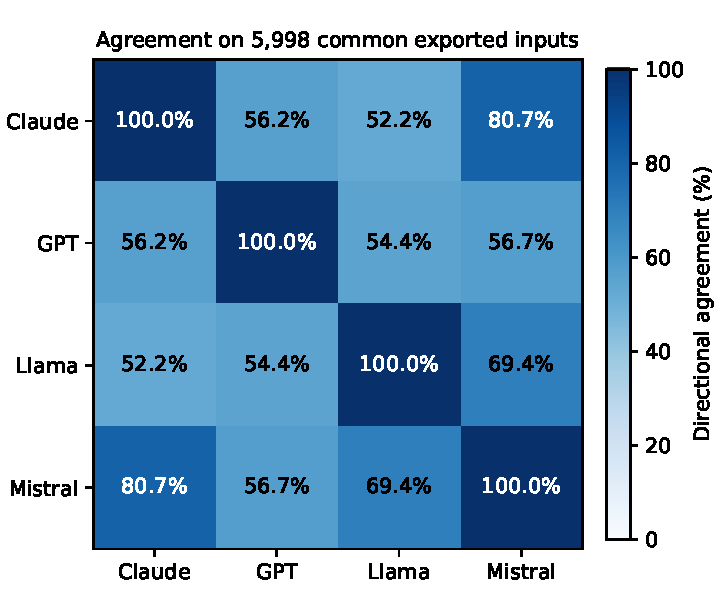
\includegraphics[width=\linewidth]{assets/common_panel_agreement.pdf}
\caption{Pairwise directional agreement on the same 5,998 exported inputs. This is response agreement, not held-out predictive accuracy.}
\label{fig:agreement}
\end{figure}

Agreement ranges from 52.20\% for Claude--Llama to 80.71\% for Claude--Mistral (Figure~\ref{fig:agreement}). The other pairs range from 54.43\% to 69.42\%. Architectural labels therefore do not imply a common degree of behavioral separation. We do not assign these agreement rates to the six simulation profiles: label agreement cannot identify their state-dependent response functions or portfolio behavior.

\subsection{Why the export is not a benchmark of profitability}
The supplied evaluation split is 97.56\% neutral and lacks GPT-4.1 mini. Of 5,197 evaluation decision identifiers, 5,186 also occur in training, despite zero exact exported-input overlap. A consensus field already present in the input matches 99.15\% of evaluation targets. The field creates a potential shortcut and complicates interpretation of the task. In 58,830 responses, the recorded response timestamp precedes the exported prompt timestamp; this may reflect later export construction and does not, by itself, prove information leakage. Excluded abstentions and errors further restrict the population being described.

Transparent controller baselines recover many supplied labels, including exit accuracy 0.9693, regime accuracy 0.9258 for a depth-eight decision tree, and risk-target $R^2=0.9812$ (coefficient of determination: the fraction of target variation explained relative to a constant prediction). Depth exploration used the supplied evaluation split, making these exploratory label-recovery diagnostics. They establish neither a fine-tuning benefit nor a trading edge. These findings motivate maintaining a strict boundary between corpus diagnostics and economic outcomes.

\section{Controlled market mechanism}
\subsection{State, decisions, and risk}
The market has one asset and $N$ agents. Index $i$ identifies an agent and integer $t$ identifies a simulation step; steps have no calibrated wall-clock duration. $P_t>0$ is the asset price, $F_t>0$ is an exogenous fundamental reference, $C_{i,t}$ is cash, and $h_{i,t}$ is signed inventory. All are scalar state variables. Equity is the marked value
\begin{equation}
 E_{i,t}=C_{i,t}+h_{i,t}P_t.
\end{equation}
Thus cash plus the current value of inventory determines the next decision's resource base. Half the agents are designated adaptive; their collective initial capital share is $\rho$ (rho), while the remaining agents receive $1-\rho$. Changing $\rho$ changes allocated capital, not agent count or real market capitalization.

The adaptive trade signal combines fundamental mispricing, the last observed price return, bounded outcome feedback, and assumed error. The error is
\begin{equation}
 e_{i,t}=\sigma_e\{\sqrt{\chi}\,z_t+\sqrt{1-\chi}\,z_{i,t}\},
\end{equation}
where $\sigma_e$ (sigma) is a chosen error scale, $\chi$ (chi) is a chosen shared-error fraction, and $z_t,z_{i,t}$ are independent standard-normal draws shared across agents or specific to agent $i$. Before clipping and feedback, two agents' errors have correlation $\chi$ when $\sigma_e>0$. This is not necessarily their action correlation. With zero error scale, changing $\chi$ has no effect.

Let $u_{i,t}\in[-1,1]$ be the clipped trade signal and $b_{i,t}\in[0,1]$ the chosen exposure fraction after drawdown attenuation. The target inventory is
\begin{equation}
 h^*_{i,t}=u_{i,t}b_{i,t}L\max(E_{i,t},0)/P_t,
\end{equation}
where $L$ is a target-exposure multiplier. Multiplying equity by signal, exposure fraction, and $L$ gives signed target currency exposure; division by price converts it to asset units. This is a simulation definition. The production field \texttt{risk\_pct} measures equity at risk and cannot be substituted directly for $b_{i,t}$.

A threshold gate freezes speculative inventory when the absolute signal is too small. Separate protective rules target zero inventory on nonpositive equity or drawdown above 50\%. These exits remain subject to the aggregate execution limit. The mechanism does not implement a broker margin model, and negative equity is recorded rather than silently removed.

\subsection{Orders, price feedback, and accounting}
Each requested inventory change is clipped to a per-step fraction of positive equity. Let $\widetilde q_{i,t}$ denote this requested quantity, $\Lambda$ (capital lambda) the fixed notional depth, and $v$ the chosen aggregate volume fraction. Executed quantity is
\begin{align}
 s_t&=\min\left(1,\frac{v\Lambda}{\max(P_t\sum_i|\widetilde q_{i,t}|,10^{-12})}\right),\\
 q_{i,t}&=s_t\widetilde q_{i,t}.
\end{align}
The scalar $s_t$ scales every request equally when gross requested notional exceeds the limit. Absolute value $|\cdot|$ counts buys and sells as positive volume; $10^{-12}$ prevents division by zero. Net flow instead uses signed quantities.

After orders are formed, the fundamental innovation and possible shock occur. Price evolves as
\begin{align}
 \log(P_{t+1}/P_t)={}&\alpha_F\log(F_{t+1}/P_t)\nonumber\\
 &+\lambda_I\psi\left(\frac{P_t\sum_iq_{i,t}}{\Lambda}\right)+\varepsilon_t.
\end{align}
Here $\log$ is the natural logarithm; $\alpha_F$ (alpha) is chosen fundamental attraction, $\lambda_I$ (lambda) chosen impact strength, $\varepsilon_t$ (epsilon) external price noise, and $\psi$ (psi) either hyperbolic tangent or a linear function. Hyperbolic tangent bounds the response to large net orders. Prices therefore respond both to external information and to actions. Orders do not observe the current step's future innovation.

Execution uses the geometric mean of old and new prices, adjusted by a signed half-spread. Fees are proportional to absolute executed notional. Cash decreases by signed transaction value plus fees; inventory increases by executed quantity. An unconstrained external dealer receives the opposite transaction and inventory, and a separate fee account receives fees. The total cash residual, including dealer and fees, and total inventory residual should be zero up to floating-point rounding. These checks validate bookkeeping, not the economic calibration of price impact.

\section{Experiments and results}
\subsection{Design and uncertainty}
The first factorial study has 32 parameter cells: two capital levels, two depths, two population sizes, two trade limits, and two shared-error settings. Three seeds and paired shock/no-shock runs yield 192 episodes. A second study uses six assumed profiles, two adaptive capital shares, two shared-error settings, 20 seeds, and both shock conditions, yielding 960 episodes. A robustness grid contributes 160 episodes across two impact laws, two exposure multipliers, two update intervals, ten seeds, and both shock conditions. The total is 1,312 episodes. Choices followed inspection of data availability; this is not a preregistered experiment.

The six profiles are a zero-error reference, low noise, high noise, stronger momentum feedback, slower adaptation, and a stronger threshold/drawdown response. They are not named language models. Some profiles change multiple parameters; comparisons are sensitivities rather than isolated causal ablations of one architecture component. Background agents use a noisy fundamental-value response. Exact settings appear in the supplement and machine-readable configurations.

We report maximum price drawdown, which is the largest fractional fall below any preceding price peak over the episode. Let $Y_r(\rho,s)$ denote this scalar outcome for seed $r$, capital share $\rho$, and shock indicator $s\in\{0,1\}$. Within each profile and error setting, the participation--shock interaction is
\begin{align}
 I_r={}&[Y_r(0.75,1)-Y_r(0.75,0)]\nonumber\\
       &-[Y_r(0.25,1)-Y_r(0.25,0)].
\end{align}
The first bracket is the shock's incremental drawdown at high participation; the second is its incremental drawdown at low participation. Positive $I_r$ means participation increases that incremental effect. It does not mean the no-shock market crashes. Negative $I_r$ can coexist with greater baseline drawdown.

Within a seed, exogenous random streams are aligned across conditions; endogenous actions are allowed to differ. Means and 95\% Student-$t$ intervals use the 20 seed-level contrasts. These intervals quantify simulation randomness conditional on the design. They exclude parameter-calibration uncertainty and do not establish population-level financial effects. No multiple-comparison adjustment is applied; the complete panel is reported rather than selecting a favorable cell.

\begin{table}[t]
\centering
\caption{Participation--shock interaction at shared-error setting 0.9, in percentage points of maximum drawdown. Intervals describe 20 simulation seeds.}
\begin{tabular}{lrr}
\toprule
Profile & Mean & 95\% interval\\\midrule
P0 Reference & 0.168 & [0.127, 0.209]\\
P1 Low noise & 0.099 & [0.063, 0.135]\\
P2 High noise & $-0.121$ & [$-0.216$, $-0.026$]\\
P3 Strong feedback & $-0.171$ & [$-0.266$, $-0.076$]\\
P4 Slow updates & $-0.040$ & [$-0.108$, 0.029]\\
P5 Selective proxy & 0.203 & [0.153, 0.254]\\
\bottomrule
\end{tabular}\label{tab:interactions}
\end{table}

\subsection{Participation does not have a uniform effect}
Table~\ref{tab:interactions} shows that participation--shock interactions change sign across assumed profiles. Under shared-error setting 0.9, the reference interaction is 0.168 percentage points and the stronger-feedback interaction is $-0.171$ percentage points. For the latter profile, however, raising participation increases no-shock maximum drawdown by 0.616 percentage points (95\% interval 0.465--0.768). The negative interaction therefore does not imply lower absolute market stress.

The selective proxy has a positive interaction of 0.203 percentage points. Its no-shock participation effect is $-0.042$ percentage points (interval $-0.080$ to $-0.004$). A policy can reduce baseline drawdown while increasing the incremental response to an imposed shock. The experiment does not support a universal resilience claim for selection. Furthermore, its gate and drawdown parameters change together, and exposure-matched controls are absent, so this is not a causal test of CMTF reasoning quality.

\begin{figure}[t]
\centering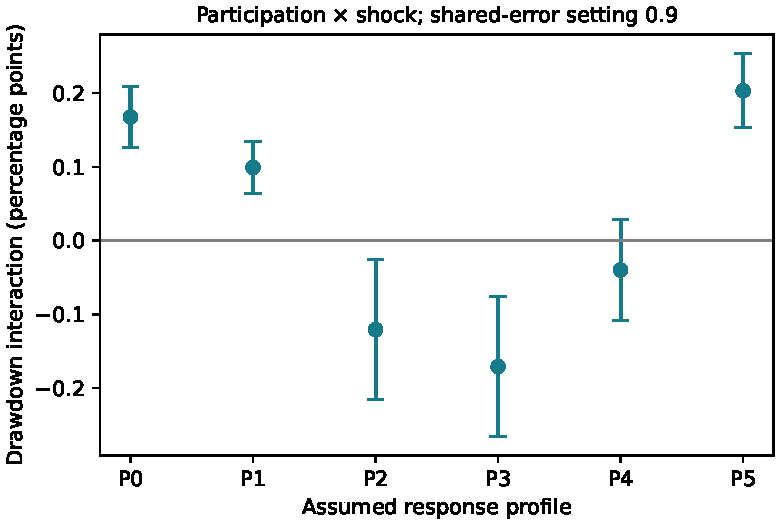
\includegraphics[width=\linewidth]{assets/profile_interactions.pdf}
\caption{Paired participation contrasts for assumed profiles. These are finite-horizon simulation sensitivities, not estimated real-market transition boundaries.}
\end{figure}

The three-seed broad grid is a mechanics check, not a precise estimate of rare-event probabilities. A 10\% drawdown indicator is available in the output, but the experiment neither calibrates a crash definition to market data nor identifies a discontinuity. The robustness grid varies implementation assumptions; it does not establish robustness to every omitted market mechanism.

\subsection{Reproducibility and historical illustration}
The simulation grids satisfy cash and inventory checks to numerical precision: the largest absolute cash residual in the broad grid is $3.73\times10^{-9}$ currency units and the inventory residual is $7.28\times10^{-12}$ asset units. The full author package executed eight notebooks with 28 code cells and no error outputs, and passed 21 contract tests. Kernel execution used one isolated in-process Jupyter kernel per notebook because socket binding was unavailable in the preparation environment.

A separate illustration uses 192 fifteen-minute XAUUSD clock points from June 29--30, with 84 fresh recorded outputs and three entry-gate points. It assumes an exposure fraction of 0.6; absent or stale information disables new speculative targets. It is an output-driven illustration plus feedback, not a complete two-role historical replay, and it is excluded from the 1,312 grid episodes.

\section{Limitations and conclusion}
The corpus audit is descriptive and relies on exported information. The original inference inputs, complete portfolio responses, and continuous broker equity ledger are unavailable. Thus neither original model-policy reproduction nor risk-adjusted alpha is established. Private-source restrictions also prevent unrestricted replication of the operational counts.

The simulator imposes fixed depth and an unconstrained dealer. It omits an order book, endogenous liquidity withdrawal, financing, calibrated margin liquidation, and real model responses to counterfactual states. Its bounded numerical adaptation is not language-model retraining. Shared noise is not shared causal-graph misspecification. The simulation measures net marked return but has no factor benchmark, so it does not measure alpha or alpha decay.

Within those limits, the study establishes a reproducible connection between evidence auditing and controlled market-feedback experiments. Observed response diversity motivates heterogeneous-policy analysis, but does not determine its parameters. Participation affects baseline stress and incremental shock response differently across assumed policies. These results support conditional mechanism analysis and explicit evidence boundaries, rather than a universal claim that adaptation stabilizes or destabilizes markets.
